\newpage
\begin{center}
  \textbf{\large 1. Постановка задачи}
\end{center}
\refstepcounter{chapter}
\addcontentsline{toc}{chapter}{1. Постановка задачи}


\section{Анализ типов датчиков углового положения и их применимость в экстремальных условиях}

Современные следящие системы, используемые в зеркальных антенных комплексах, требуют высокой точности и надежности измерений углового положения. 
Для решения этой задачи применяются датчики различных типов, каждый из которых обладает уникальными характеристиками, ограничениями и областью применения. 
Рассмотрим основные категории таких устройств.

\textbf{Oптические энкодеры} 
  
   Эти устройства являются наиболее распространённым решением для измерения угловых перемещений. Принцип действия основан на регистрации светового потока, проходящего через перфорированный диск, 
  закреплённый на валу объекта. Благодаря фотодетекторам, преобразующим световые импульсы в электрические сигналы, можно точно определять положение и скорость вращения.
   Основное достоинство оптических энкодеров заключается в высокой точности (до нескольких угловых секунд) и хорошей разрешающей способности. 
   Однако их работа ограничена условиями эксплуатации: повышенная влажность и температура приводят к образованию конденсата на оптике, 
   что негативно влияет на сигнал и даже может вызвать выход из строя электронного оборудования. 
   Длительное использование в суровых условиях среды ускоряет износ механических элементов, например, подшипников. В связи с этим возникает необходимость в поддержании нормальных климатических условий,
   что может быть трудновыполнимой задачей (см. рис.~\ref{OpuInSnow}). 

  \begin{figure}[!t]
    \centering
    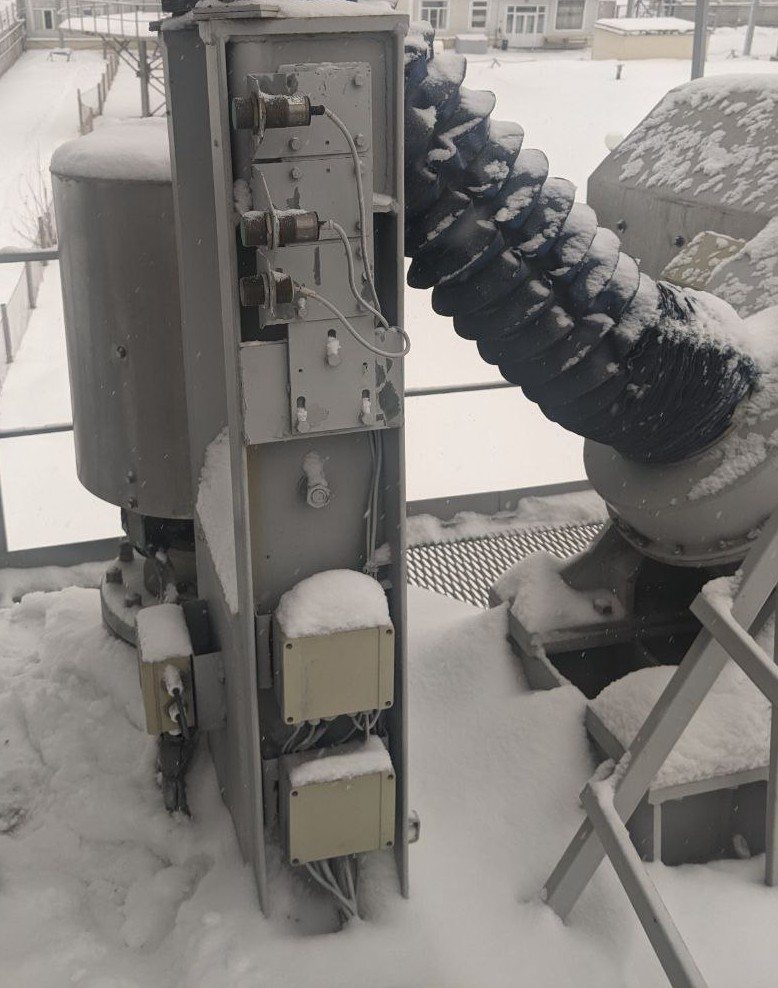
\includegraphics[width=150mm]{OPU.JPG}
    \caption{Заснеженные датчики}
    \label{OpuInSnow}
  \end{figure}

  \newpage
  \textbf{Магнитные энкодеры}
  
  Альтернатива оптическим устройствам — магнитные энкодеры, например модель ЛИР-ММ137А, 
  которые используют датчики Холла и магнитные редукторы. Угол поворота измеряется изменением магнитного поля, создаваемого многополюсным магнитом, 
  благодаря чему исключается потребность в оптических компонентах. 
  Это значительно улучшает стойкость к загрязнениям и влагозащиту. 
  Тем не менее, электронные схемы обработки сигналов остаются чувствительными элементами конструкции. 
  Так, низкие температуры вызывают образование льда на проводах и контакты подвергаются коррозии, что ведёт к ошибкам измерений. 
  Помимо этого, мощные внешние магнитные поля (например, излучения антенн) оказывают влияние на показания прибора (см. рис.~\ref{SnowAntenna}).
  \begin{figure}[!t]
    \centering
    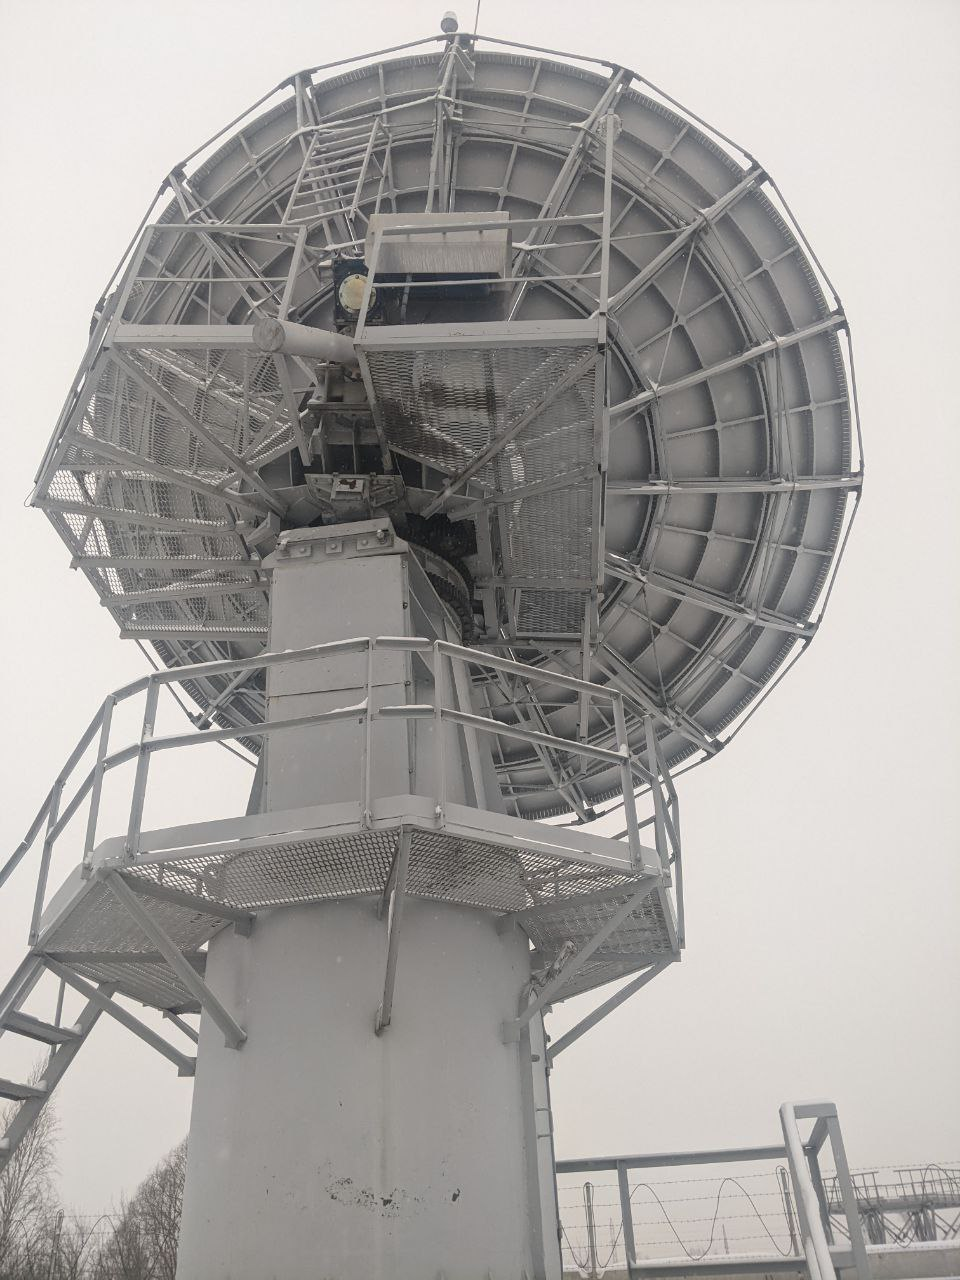
\includegraphics[width=150mm]{SnowAntenna.JPG}
    \caption{Антенная система в снегу}
    \label{SnowAntenna}
  \end{figure}


\newpage
\section{Индукционные датчики углового положения: сельсины, вращающиеся трансформаторы и индуктосины}

Индукционные датчики углового положения, основанные на принципах электромагнитной индукции, являются ключевыми компонентами высоконадежных следящих систем. 
К этой категории относятся: 
\begin{itemize} \item сельсины \item вращающиеся трансформаторы (ВТ) \item  индуктосины \end{itemize}

\textbf{Сельсины}

Сельсины — это индукционные машины, преобразующие механический угол поворота в электрический сигнал. Они состоят из пары синхронизированных устройств: датчика (сельсин-датчика) 
и приемника (сельсин-приемника). При изменении угла ротора датчика возникает рассогласование, которое преобразуется в сигнал ошибки, управляющий исполнительным механизмом.
Основное преимущество сельсинов — высокая надежность и устойчивость к вибрациям, влаге и температурным перепадам. Однако их точность (±10–15 угловых минут) 
и быстродействие уступают современным требованиям, что ограничивает их применение в высокоточных системах наведения.

\textbf{Вращающиеся трансформаторы (ВТ)}

Вращающиеся трансформаторы — это бесконтактные индукционные датчики, генерирующие сигналы, пропорциональные синусу и косинусу угла поворота вала. 
Благодаря отсутствию электронных компонентов в активной зоне, ВТ обладают исключительной устойчивостью к экстремальным условиям: температурам от -60°C до +150°C, 
вибрациям до 100 g и воздействию агрессивных сред.
Точность стандартных моделей ВТ, таких как ВТ-5 КФ3.031.055, достигает ±2 угловых минут без дополнительных доработок, что удовлетворяет требованиям большинства антенных систем. 
Однако такие устройства, разработанные для военного применения, отличаются высокой стоимостью и длительными сроками поставки (до 12–18 месяцев), 
что делает их малопригодными для гражданских проектов.

\textbf{Индуктосины}

Индуктосины — это прецизионные индукционные датчики, работающие по принципу изменения взаимной индуктивности между статором и ротором. Они обеспечивают точность до ±1 угловой секунды, 
что делает их привлекательными для задач сверхточного позиционирования. Однако сложность конструкции, высокая стоимость и необходимость использования специализированной электроники для обработки 
сигналов ограничивают их применение в массовых системах.

\section{Проблема выбора доступных решений}
Для гражданских и коммерческих проектов критически важно использование серийно выпускаемых компонентов, которые сочетают надежность, точность и доступность. 
В этом контексте перспективными являются вращающиеся трансформаторы, выпускаемые в стандартизированных корпусах, таких как ROD 426 и ROD 456 от компании Heidenhain. 
Эти габариты соответствуют общепромышленным стандартам, что обеспечивает:

\begin{itemize} 
  \item Совместимость с широким спектром монтажных узлов и редукторов.
  \item Упрощение замены при модернизации систем.
  \item Снижение затрат за счет массового производства и доступности на рынке.
\end{itemize}

Например, ВТ в корпусе ROD 456, несмотря на меньшую точность (±5 угловых минут), могут быть дополнены двухотсчетной схемой измерения, 
что позволяет повысить разрешающую способность до требуемых значений (±2’).


\section{Что выбрали}

Для повышения надежности электропривода, в качестве измерительных элементов углов рассогласования предлагается использовать общепромышленные и доступные 
синусно-косинусные вращающиеся трансформаторы (резольверы) А12, А13, А27, А29, А40, А42 такие как ЛИР-ДР158А. Благодаря своей простой конструкции, 
такие датчики углового положения могут без сбоев работать в условиях конденсата. Поскольку погрешность таких датчиков углового положения составляет ±10', 
в целях увеличения точности, измерители углов рассогласования следует выполнять по двухотсчетной схеме с грубым и точным отсчетом и редукцией 1:30. \ref{Reductor.png} 

  \begin{figure}[!t]
    \centering
    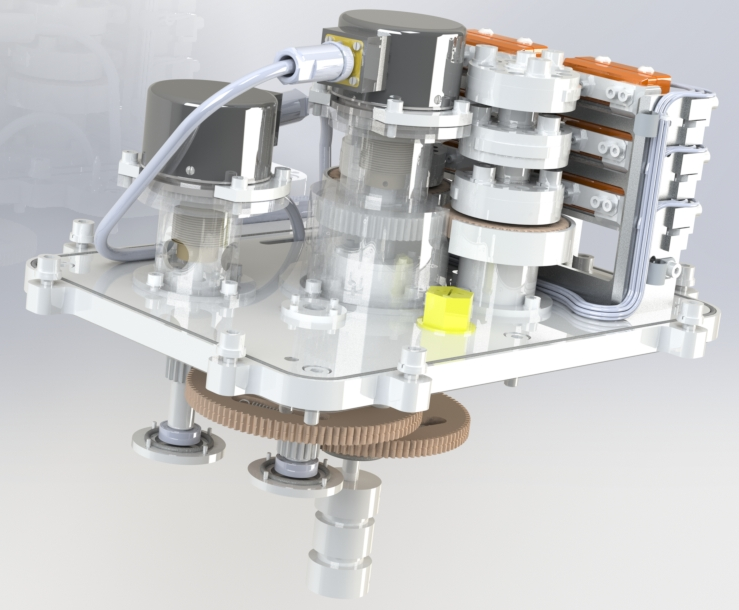
\includegraphics[width=150mm]{Reductor.png}
    \caption{Редуктор УМ}
    \label{Reductor}
  \end{figure}

\section*{Определение погрешностей многоступенчатого передаточного механизма}

Погрешность каждой передачи приводится к выходному $n$-му звену, будучи поделена на передаточное отношение от данной передачи до выходного звена. При наличии паразитных звеньев их следует учитывать дважды -- как ведомое в паре с предыдущим и ведущее в паре с последующим звеном кинематической цепи.

\subsection*{Максимальная кинематическая погрешность $\delta\phi_{\Sigma \text{max}}$ и максимальный кинематический мертвый ход $j\phi_{\Sigma \text{max}}$}

\begin{equation}
    \delta\phi_{\Sigma \text{max}} = \delta\phi_{\text{max}12} + \delta\phi_{\text{max}34} + \dots + \delta\phi_{\text{max}(n-1)n}, \quad y \geq \pi. \quad \text{МКХ.} \tag{6.53}
\end{equation}

\begin{equation}
    j\phi_{\Sigma \text{max}} = \frac{j_{\text{max}12} + j_{\text{max}34} + \dots + j_{\text{max}(n-1)n}}{i_m}, \quad y \geq \pi. \quad \text{МКХ.} \tag{6.54}
\end{equation}

где $n$ -- номер выходного колеса $z_n$.

\subsection*{Минимальная кинематическая погрешность $\delta\phi_{\Sigma \text{min}}$ и минимальный кинематический мертвый ход $j\phi_{\Sigma \text{min}}$}

\begin{equation}
    \delta\phi_{\Sigma \text{min}} = \delta\phi_{\text{min}12} + \delta\phi_{\text{min}34} + \dots + \delta\phi_{\text{min}(n-1)n}, \quad y \geq \pi. \quad \text{МКХ.} \tag{6.55}
\end{equation}

\begin{equation}
    j\phi_{\Sigma \text{min}} = \frac{j_{\text{min}12} + j_{\text{min}34} + \dots + j_{\text{min}(n-1)n}}{i_m}, \quad y \geq \pi. \quad \text{МКХ.} \tag{6.56}
\end{equation}

